\documentclass[border={2pt 2pt 2pt 2pt}]{standalone}

\usepackage{amssymb}
\usepackage{tikz}
\usetikzlibrary{arrows, automata, positioning, shapes}
\usetikzlibrary{arrows.meta}

\begin{document}	\centering
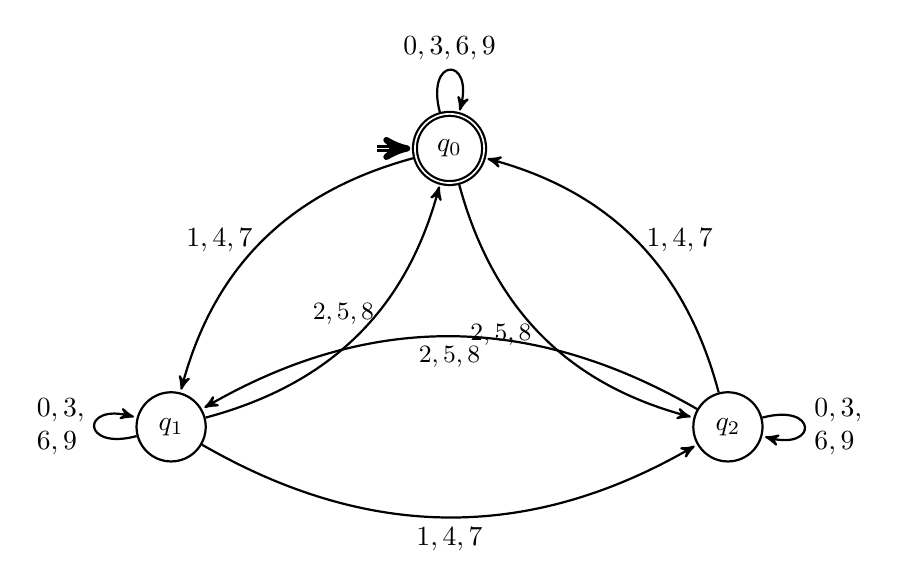
\begin{tikzpicture}[
	->,
	>=stealth',
	shorten >=1pt,
%	auto,
	node distance=5cm,
	initial text=,
	thick
]

\tikzstyle{every initial by arrow} = [->, double];

 \node [state, initial, accepting] (q_0)                        {$q_0$};
 \node [state]                     (q_1) [below left of = q_0]  {$q_1$};
 \node [state]                     (q_2) [below right of = q_0] {$q_2$};

 \path [->] (q_0) edge [bend right] node [left]              {$1,4,7$}                 (q_1)
                  edge [loop above] node [above]             {$0,3,6,9$}               ()
                  edge [bend right] node [left]              {{\small $2,5,8$}}        (q_2)
            (q_1) edge [bend right] node [below]             {$1,4,7$}                 (q_2)
                  edge [loop left]  node [left, align=left]  {$0,3,$ \\ $6,9$}         ()
                  edge [bend right] node [above]             {{\small $2,5,8$} \ \ \ } (q_0)
            (q_2) edge [bend right] node [right]             {$1,4,7$}                 (q_0)
                  edge [loop right] node [right, align=left] {$0,3,$ \\ $6,9$}         ()
                  edge [bend right] node [below]             {{\small $2,5,8$}}        (q_1);

\end{tikzpicture}
\end{document}
